\subsection{Primo sprint}

\begin{minipage}{\textwidth}
Di seguito è riportata la distribuzione delle ore per ciascun membro del team, accumulate in totali per persona e per ruolo:
\begin{table}[H]
  \begin{tabularx}{\textwidth}{|c|*{6}{>{\centering}X|}c|}
    \hline
    \multicolumn{8}{|c|}{\textbf{Consuntivo orario}} \\
    \hline
    \textbf{Membro del team} & \textbf{Re} & \textbf{Am} & \textbf{An} & \textbf{Pt} & \textbf{Pr} & \textbf{Ve} & \textbf{Totale per persona} \\
    \hline
    Cavalli Riccardo & 7 & 0 & 0 & 0 & 0 & 0 & 7 \\
    \hline
    Pianon Raul & 0 & 0 & 0 & 0 & 0 & 8 & 8 \\
    \hline
    Dall'Amico Martina & 0 & 0 & 8 & 0 & 0 & 0 & 8 \\
    \hline
    Cristo Marco & 0 & 0 & 7 & 0 & 0 & 0 & 7 \\
    \hline
    Lewental Sebastiano & 0 & 0 & 7 & 0 & 0 & 0 & 7 \\
    \hline
    Zecchinato Mattia & 0 & 0 & 1 & 6 & 0 & 0 & 7 \\
    \hline
    Stocco Tommaso & 0 & 6 & 0 & 0 & 0 & 0 & 6 \\
    \hline
    \textbf{Totale per ruolo} & 7 & 6 & 23 & 6 & 0 & 8 & \textbf{50} \\
    \hline
  \end{tabularx}
  \caption{Sprint 1 - Consuntivo orario}
\end{table}
\end{minipage}

\begin{figure}[H]
  \centering
  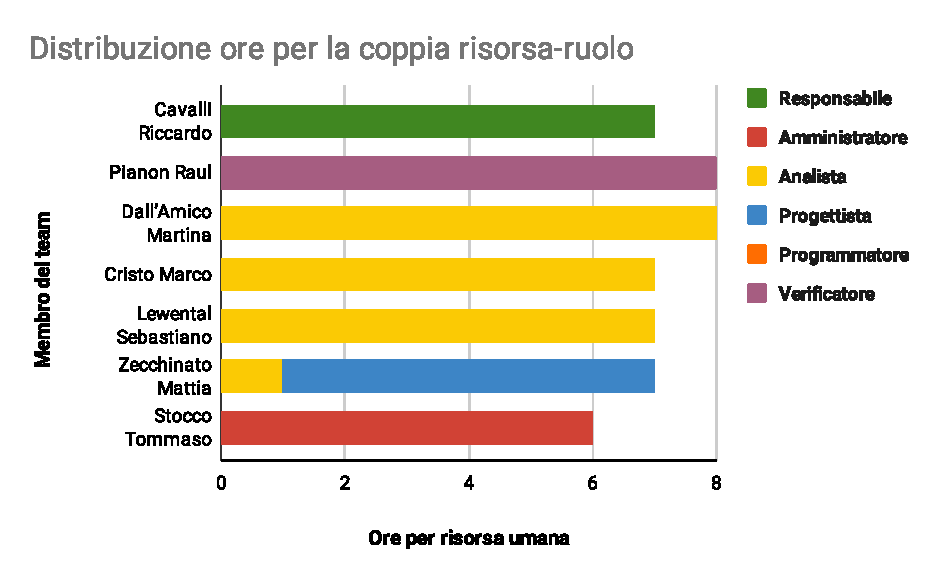
\includegraphics[width=0.90\textwidth]{assets/Consuntivo/Sprint-1/distribuzione_ore_risorsa_ruolo.pdf}
  \caption{Sprint 1 - Istogramma della distribuzione oraria per la coppia risorsa-ruolo}
\end{figure}

\begin{figure}[H]
  \centering
  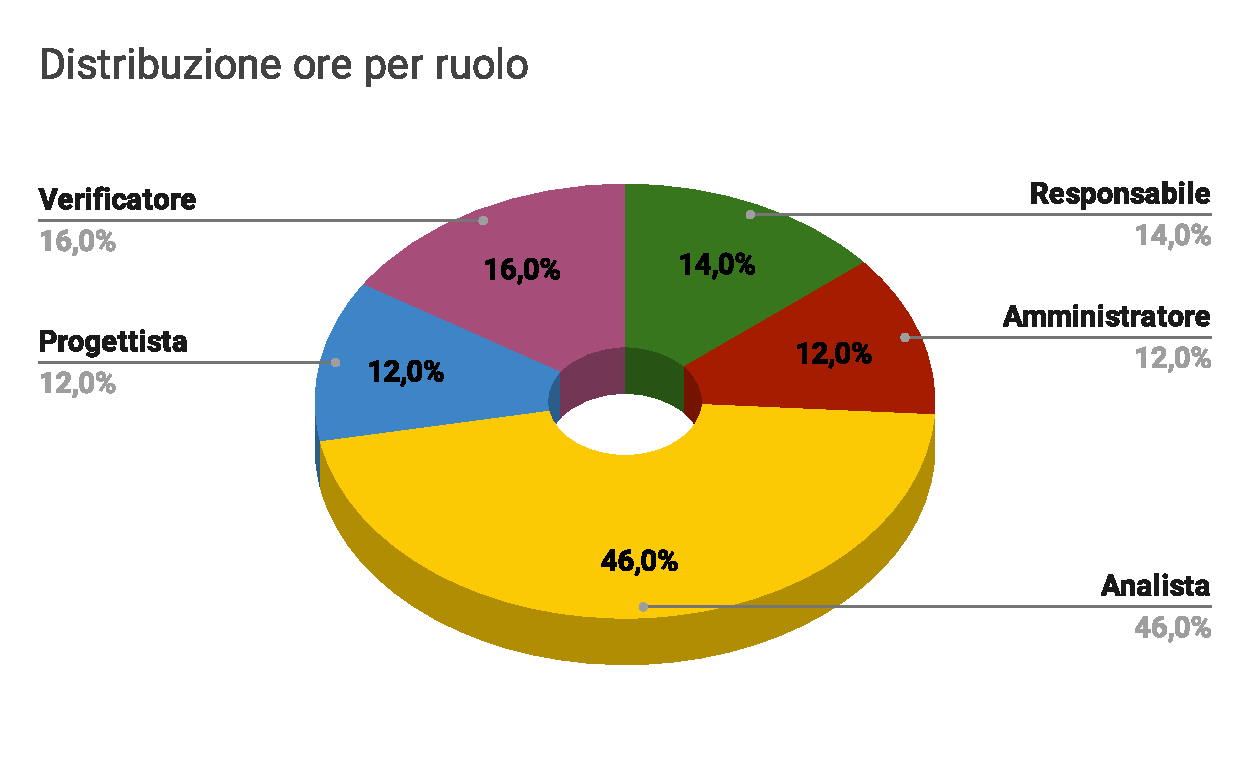
\includegraphics[width=0.90\textwidth]{assets/Consuntivo/Sprint-1/distribuzione_ore_ruolo.pdf}
  \caption{Sprint 1 - Areogramma della distribuzione oraria per ruolo}
\end{figure}

\begin{minipage}{\textwidth}
Di seguito è riportato il consuntivo economico del primo \glossario{sprint}:
\begin{table}[H]
\begin{adjustwidth}{-0.5cm}{-0.5cm}
  \centering
  \begin{tabular}{|P{2.9cm}|P{2.3cm}|P{2.5cm}|P{2.3cm}|>{\arraybackslash}P{2.5cm}|}
    \hline
    \multicolumn{5}{|c|}{\textbf{Consuntivo economico}} \\
    \hline
    \textbf{Ruolo} & \textbf{Ore per ruolo} & \textbf{Delta ore preventivo - consuntivo} & \textbf{Costo (in \texteuro)} & \textbf{Delta costo preventivo - consuntivo (in \texteuro)} \\
    \hline
    Responsabile & 7 & 0 & 210,00 & 0,00 \\
    \hline
    Amministratore & 6 & 0 & 120,00 & 0,00 \\
    \hline
    Analista & 23 & +4 & 575,00 & +100,00 \\
    \hline
    Progettista & 6 & +1 & 150,00 & +25,00 \\
    \hline
    Programmatore & 0 & 0 & 0,00 & 0,00 \\
    \hline
    Verificatore & 8 & 0 & 120,00 & 0,00 \\
    \hline
    \textbf{Totale} & \textbf{50} & +5 & \textbf{1.175,00} & +125,00 \\
    \hline
    \textbf{Restante} & 587 & / & 11.845,00 & / \\
    \hline
    \textbf{Sprint pregressi} & 0 & / & 0,00 & / \\
    \hline
  \end{tabular}
  \caption{Sprint 1 - Consuntivo economico}
\end{adjustwidth}
\end{table}
\end{minipage}

\begin{figure}[H]
  \centering
  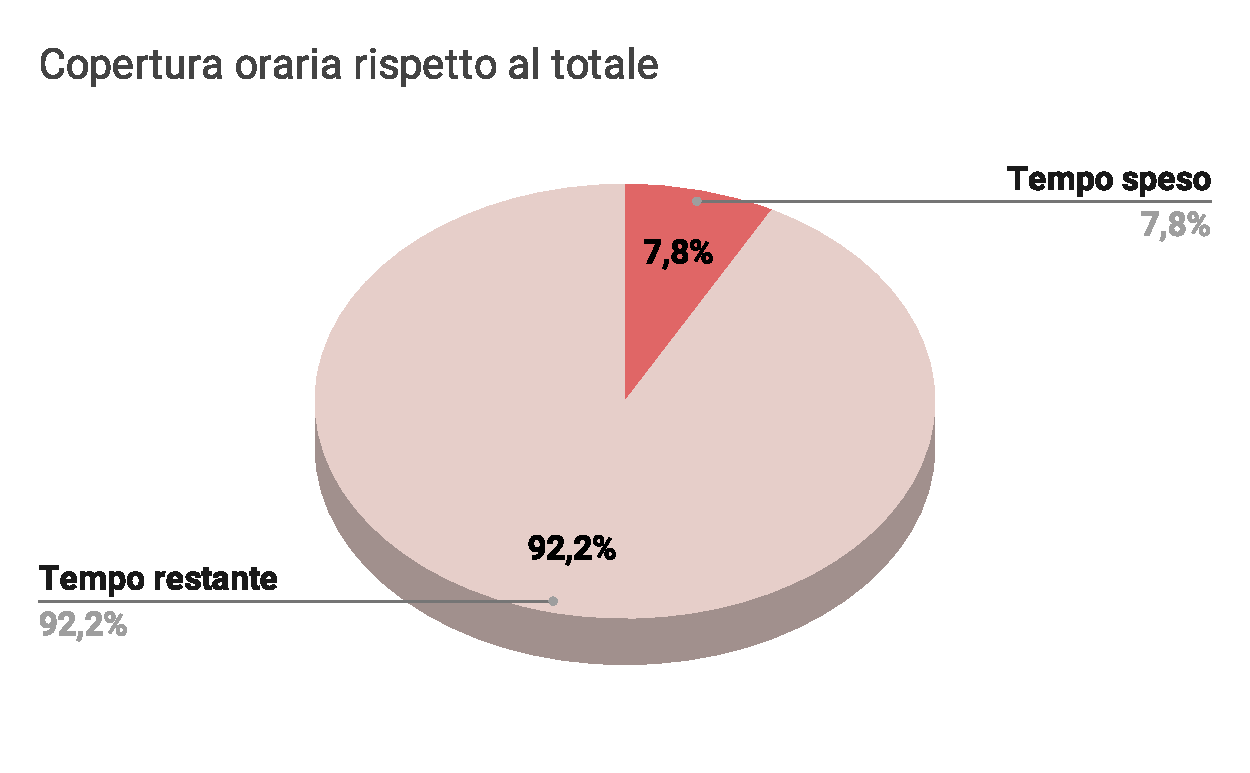
\includegraphics[width=0.90\textwidth]{assets/Consuntivo/Sprint-1/copertura_oraria.pdf}
  \caption{Sprint 1 - Areogramma del tempo speso (in ore) rispetto al totale}
\end{figure}

\begin{figure}[H]
  \centering
  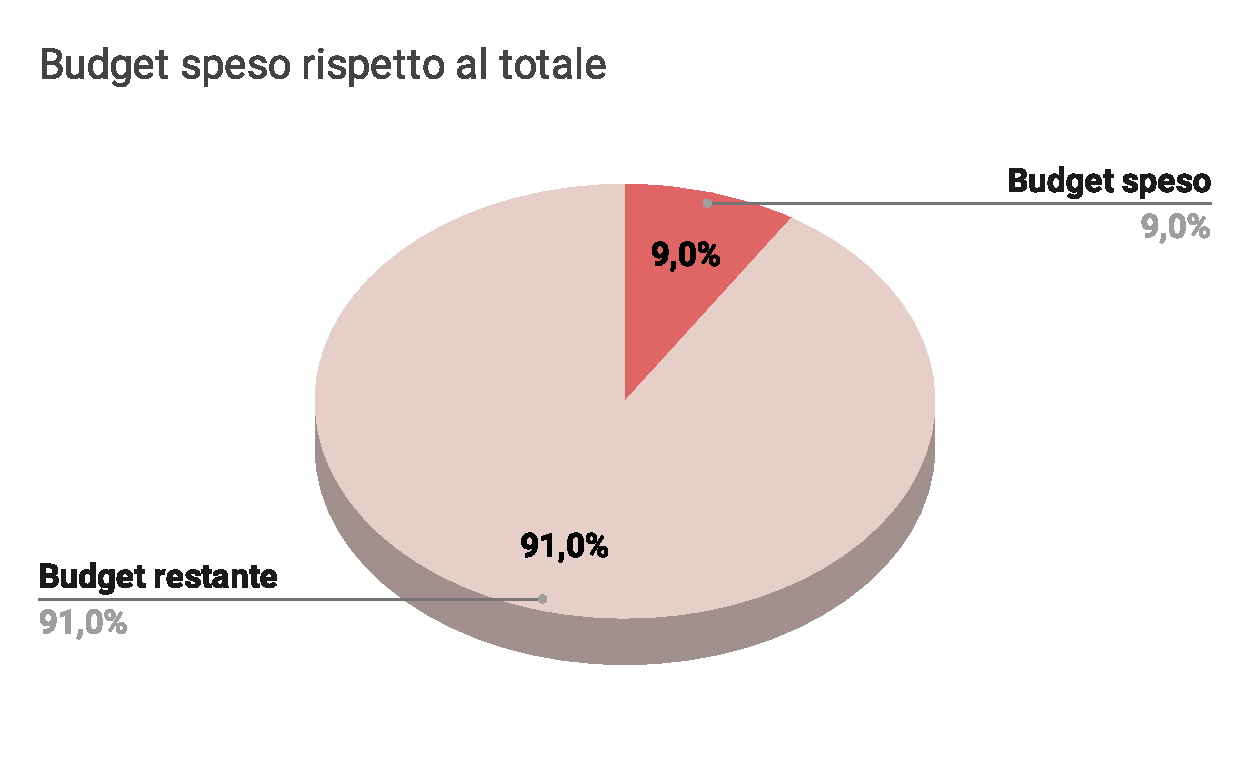
\includegraphics[width=0.90\textwidth]{assets/Consuntivo/Sprint-1/budget_speso.pdf}
  \caption{Sprint 1 - Areogramma del budget speso rispetto al totale}
\end{figure}


\begin{minipage}{\textwidth}
  Di seguito sono riportate le ore rimanenti per la coppia risorsa-ruolo:
  \begin{table}[H]
    \begin{tabularx}{\textwidth}{|c|*{6}{>{\centering}X|}c|}
      \hline
      \multicolumn{8}{|c|}{\textbf{Ore rimanenti per la coppia risorsa-ruolo}} \\
      \hline
      \textbf{Membro del team} & \textbf{Re} & \textbf{Am} & \textbf{An} & \textbf{Pt} & \textbf{Pr} & \textbf{Ve} & \textbf{Totale per persona} \\
      \hline
      Cavalli Riccardo & 2 & 8 & 9 & 23 & 22 & 20 & 84 \\
      \hline
      Pianon Raul & 9 & 8 & 9 & 23 & 22 & 12 & 83 \\
      \hline
      Dall'Amico Martina & 9 & 8 & 1 & 23 & 22 & 20 & 83 \\
      \hline
      Cristo Marco & 9 & 8 & 2 & 23 & 22 & 20 & 84 \\
      \hline
      Lewental Sebastiano & 9 & 8 & 2 & 23 & 22 & 20 & 84 \\
      \hline
      Zecchinato Mattia & 9 & 8 & 8 & 17 & 22 & 20 & 84 \\
      \hline
      Stocco Tommaso & 9 & 2 & 9 & 23 & 22 & 20 & 85 \\
      \hline
      \textbf{Totale per ruolo} & 56 & 50 & 40 & 155 & 154 & 132 & \textbf{587} \\
      \hline
    \end{tabularx}
    \caption{Sprint 1 - Ore rimanenti per la coppia risorsa-ruolo}
  \end{table}
\end{minipage}

\subsubsection{Revisione delle attività}

Nel corso del primo \glossario{sprint}, il team ha svolto le seguenti attività:
\begin{itemize}
  \item Stesura iniziale del \PdP;
  \item Scelta del modello di sviluppo;
  \item Pianificazione e preventivo del secondo \glossario{sprint};
  \item \AdR\ e definizione dei primi \glossario{casi d'uso};
  \item Individuazione degli \glossario{attori} coinvolti nel sistema e delle loro caratteristiche;
  \item Analisi dei rischi tecnologici e organizzativi;
  \item Composizione preliminare del \glossario{dizionario dati};
  \item Raccolta dei termini da inserire nel \Gls;
  \item Miglioramento del \WoW\ e automazione delle procedure con relativa stesura delle \NdP;
  \item Valutazione di eventuali alternative all'\glossario{Issue Tracking System} di \glossario{GitHub}.
\end{itemize}

\subsubsection{Retrospettiva}
\par Di seguito sono riportati i risultati del questionario di valutazione dello \glossario{sprint}, realizzato dal responsabile in carica per supportare la fase di \glossario{retrospettiva}:
\begin{itemize}
  \item Organizzazione dello \glossario{sprint} - Valutazione: 7,5;
  \item Conduzione dei meeting interni - Valutazione: 7,5;
  \item Conduzione dei meeting esterni - Valutazione: 8;
  \item Impegno e partecipazione dei singoli membri - Valutazione: 7;
  \item Non tutti i membri del team erano a conoscenza delle proprie mansioni;
  \item La numerosità delle riunioni è adeguata;
  \item Le riunioni sono state organizzate quasi sempre con il giusto preavviso;
  \item Da migliorare il rapporto ore spese/ore produttive.
\end{itemize}

\vspace{0.5\baselineskip}
\par A seguire le \textbf{analisi a posteriori} del primo \glossario{sprint}:
\begin{itemize}
  \item Le valutazioni raccolte dal team hanno evidenziato una pianificazione idonea ma non esaustiva. Di conseguenza, la transizione da un'attività a quella successiva non è sempre stata immediata, e ciò ha portato a delle fasi, seppur brevi, di stallo. Per tale motivo è stata registrata una discrepanza di 5 ore produttive rispetto a quanto definito nel preventivo;
  \item Inoltre, il gruppo ha ritenuto di aver sovrastimato il carico di lavoro per alcuni ruoli, in particolare l'analista e il progettista, a cui sono state assegnate 34 ore produttive totali. A posteriori, il team avrebbe preferito rimuovere una risorsa dal ruolo di analista, per assegnarla a mansioni impegnative come l'amministratore e il responsabile;
  \item Per via di una pianificazione non dettagliata, dell'inesperienza nell'\AdR\ e di una distribuzione non omogenea delle ore, il gruppo ha performato al di sotto delle aspettative in determinati ruoli. Tuttavia, la mancanza di uniformità nella ripartizione dei ruoli ha contruibuito alla creazione di micro-gruppi autonomi. Ciò ha favorito la condivisione delle conoscenze e la collaborazione, riducendo al minimo le perdite dal punto di vista dell'intensità di lavoro, che sarebbero altrimenti risultate pregiudizievoli;
  \item Il team ha riscontrato un feedback positivo per quanto riguarda l'organizzazione e la conduzione delle riunioni. Al contrario, sono stati rilevati come aspetti da migliorare la coesione interna e il rendimento delle singole risorse;
  \item Durante il primo \glossario{sprint}, il progettista ha lavorato a stretto contatto con il team di analisti. Perciò, la definizione del \glossario{dizionario dati} è passata in secondo piano rispetto al delineamento dell'architettura generale dell'applicazione. Questo ha comportato un aggiornamento della pianificazione, al fine di spostare la stesura del \glossario{dizionario dati} alla prossima iterazione;
  \item La redazione del verbale esterno del 3 aprile 2024 ha subito un ritardo per via dell'inesperienza del team nell'uso di \glossario{LaTeX}. Dal prossimo \glossario{sprint}, il gruppo si prefigge di aggiornare il template \glossario{LaTeX} (con l'aggiunta di parametri e comandi predefiniti) per velocizzare la stesura dei documenti. Inoltre, si è deciso di rendere il contenuto dei verbali più asciutto e conciso. Ciò non significa però che si debba rinunciare a un resoconto dettagliato delle riunioni;
  \item Gli ostacoli principali dal punto di vista organizzativo sono scaturiti dalla mancanza di una lista puntuale delle attività da svolgere. L'\glossario{Issue Tracking System} di \glossario{GitHub} non è stato sufficiente a garantire una corretta e completa gestione dei task. Per tale motivo, il team ha deciso di valutare l'adozione di \glossario{Jira} come \glossario{ITS}. Gli strumenti sviluppati da Atlassian, difatti, sembrano essere maggiormente orientati verso il modello \glossario{Agile}; inoltre, sono disponibili funzionalità come il calendario e la timeline che offrono una visione d'insieme del progetto e di eventuali ritardi;
  \item Nella prima metà dello \glossario{sprint}, la risorsa impiegata nel ruolo di verificatore ha ricevuto un carico di lavoro inferiore rispetto a quanto pianificato. Durante la riunione di \glossario{retrospettiva}, il team ha convenuto che, in futuro, le ore potenzialmente “dissipate” potrebbero essere utilizzate in modo produttivo se impiegate in un ruolo diverso.
\end{itemize}

\subsubsection{Aggiornamento pianificazione e preventivo}
\par Il team ha definito un piano d'azione per migliorare l'organizzazione e la produttività del prossimo \glossario{sprint}:
\begin{itemize}
  \item Definire una "To-Do List" più precisa;
  \item Organizzare riunioni brevi e mirate;
  \item Interazione più frequente tra il responsabile e il team di sviluppo;
  \item Pianificare lo studio delle tecnologie in maniera graduata;
  \item Verificare costantemente il progresso delle attività e la documentazione di progetto;
  \item Programmare un incontro in presenza con cadenza mensile;
  \item Sinergia tra ruoli con funzioni complementari;
  \item Sfruttare l'esperienza acquisita da chi ricopriva un ruolo in precedenza;
  \item Possibilità di assumere più ruoli durante uno \glossario{sprint};
  \item Distribuzione più omogenea delle ore tra i ruoli;
  \item Proseguire sulla strada dei micro-gruppi.
\end{itemize}

\paragraph*{Pianificazione futura:}
\par Come riportato nelle analisi a posteriori, il team ha posticipato la stesura del \glossario{dizionario dati} al secondo \glossario{sprint}. Inoltre, il gruppo ha dovuto riconsiderare l’idea di partenza in merito allo studio delle tecnologie. Nella fase di candidatura, infatti, il team aveva stabilito che, nell’arco del primo \glossario{sprint}, tutti i membri del gruppo avrebbero dovuto approfondire i linguaggi e le librerie proposte, specialmente \glossario{txtai}.

\vspace{0.5\baselineskip}
\par Questa pianificazione preliminare, tuttavia, non teneva conto delle attività di natura organizzativa, proprie del responsabile e dell’amministratore. Inoltre, la stesura della documentazione ha coperto la quasi totalità dello \glossario{sprint}. Lo studio delle tecnologie è stato quindi spostato al prossimo periodo. In definitiva, la pianificazione del secondo \glossario{sprint} viene aggiornata con le seguenti attività:
\begin{itemize}
  \item Definizione del \glossario{dizionario dati};
  \item Studio di \glossario{txtai} e creazione di programmi per testare le funzionalità della libreria.
\end{itemize}

\vspace{0.5\baselineskip}
\par Durante la riunione di \glossario{retrospettiva}, il team ha valutato anche la creazione di un file di configurazione da caricare nel \glossario{repository} documentale di \glossario{GitHub}. Attualmente, i documenti in formato PDF vengono generati in locale e caricati manualmente sul \glossario{repository} di vetrina. Tale operazione, però, è poco scalabile e vincolata alle prestazioni delle singole macchine. Viceversa, il file di configurazione consentirebbe di automatizzare la compilazione e la distribuzione dei documenti.


\paragraph*{Preventivo "a finire" (\sezione{sec:stima_temporale}):}
\par Riguardo al ruolo di analista, le ore non impiegate saranno reinvestite nello \glossario{sprint} a ridosso della \glossario{RTB}, al fine di rivedere i \glossario{casi d'uso} e apportare dei miglioramenti formali al documento di \AdR. L'ora produttiva di progettista, invece, sarà assegnata nel quarto \glossario{sprint}, per supportare lo sviluppo dell'interfaccia grafica.

\vspace{0.5\baselineskip}
\par Durante la \glossario{retrospettiva}, il team ha evidenziato anche la necessità di ottimizzare la fase di approvazione delle modifiche. Di conseguenza, si è deciso di aggiungere una risorsa umana al ruolo di verificatore nel prossimo \glossario{sprint}. Relativamente al calendario di massima del progetto, il gruppo non ha ritenuto di dover rielaborare la data stimata per la \glossario{RTB}. Nei prossimi \glossario{sprint}, invece, verrà valutata la possibilità di designare alcune ore di progettista al ruolo di amministratore.

\paragraph*{Gestione dei rischi (\sezione{sec:analisi_rischi}):}
\par Nel corso del primo \glossario{sprint}, il team ha riscontrato l'affioramento di un rischio inatteso:
\begin{itemize}
  \item \textbf{Risorse disponibili ma non impiegate:} il gruppo non ha elaborato un numero sufficiente di documenti affinchè il verificatore potesse mantenere un'intensità di lavoro elevata. Pertanto, la media produttiva giornaliera della risorsa impiegata in tale ruolo non è rimasta costante. Dato il cospicuo numero di attività da svolgere, il team ritiene che la staticità dei ruoli sia inconciliabile con la metodologia scelta. Nella sezione di analisi dei rischi è stato quindi aggiunto un ulteriore rischio organizzativo. Secondo quanto stimato dal gruppo, la probabilità che il rischio si verifichi è alta, mentre il grado di criticità è medio. A partire dal prossimo periodo, il team si pone come obiettivo rendere più dinamica l'assegnazione delle attività.
\end{itemize}

\vspace{0.5\baselineskip}
\par Durante lo \glossario{sprint}, alcune contromisure si sono rivelate insufficienti a mitigare i rischi individuati in fase di pianificazione. Perciò il gruppo ha deciso di aggiornare l'analisi dei rischi; in particolare, sono stati rivalutati i seguenti rischi:
\begin{itemize}
  \item \textbf{Scarso know-how tecnologico:} il team ha aggiornato la probabilità di occorrenza, spostandola da "media" ad "alta". Dal prossimo \glossario{sprint}, infatti, il gruppo prevede di introdurre, oltre a \glossario{LaTeX} e \glossario{Docker}, altre tecnologie come \glossario{Jira}, \glossario{txtai}, \glossario{YAML}, \glossario{JSON} e \glossario{Python}. Le misure precedentemente adottate si sono rivelate incomplete poiché non consideravano la possibilità di lavorare in coppia per risolvere un problema. Inoltre, il team ritiene di non dover sospendere il lavoro per apprendere nuove tecnologie, assegnando piuttosto lo studio a un gruppo ristretto di risorse. Tale gruppo terrà poi un workshop per condividere le conoscenze. In aggiunta, il team ha migliorato le strategie di rilevamento del rischio tecnologico, introducendo la \glossario{continuous integration}. Le modifiche complete sono visibili nella sezione di analisi dei rischi;
  \item \textbf{Rischio legato all'inesperienza:} tale rischio, considerato troppo vago e dispersivo, è stato rinominato in "Sottostima delle risorse necessarie per un'attività". Per migliorarne la gestione, il team ha definito con maggior rigore il processo di suddivisione dei task in sotto-attività. Le misure di mitigazione, documentate nella sezione di analisi dei rischi, hanno l'obiettivo di ridurre gli impatti negativi sui task successivi.
\end{itemize}


\vspace{0.5\baselineskip}
\par Durante il primo \glossario{sprint}, alcune contromisure si sono rivelate utili a mitigare i rischi individuati in fase di pianificazione. In particolare:
\begin{itemize}
  \item \textbf{Malfunzionamenti software:} Collegarsi durante le riunioni è stato inizialmente complesso a causa della connessione a internet dei membri del gruppo o delle piattaforme del servizio. Il rischio è stato mitigato rimandando l'inizio di alcune riunioni, cercando nuove piattaforme e programmando gli incontri per tempo in modo da permettere i membri del gruppo di andare in luoghi con una buona connesione;
  \item \textbf{Rischi relativi alla collaborazione:} Collaborare con delle persone con cui non si ha mai lavorato prima è stato complesso non sapendo le rispettive tempistiche, competenze e modalità di interazione. Per arginare la problematica le riunioni inizialmente sono state lunghe e ognuno ha convidiso la sua visione o ciò che aveva compreso ad ogni avanzamento.
\end{itemize}
